\section{Paths}
\label{sec:paths}





\begin{frame}
	%
	\frametitle{Paths: brief introduction}
	%
	\begin{itemize}
		%
		\item connect two points (e.g.\ with arrows)
		%
		\item connect two nodes (e.g.\ with arrows)
		%
		\item draw some useful lines (e.g.\ axes)
		%
		\item fully customizable
		%
	\end{itemize}
	%
	(example file: \url{./Sources/paths__scalar_linear_function.tex})
	%
	
\begin{figure}[!htb]
\begin{center}
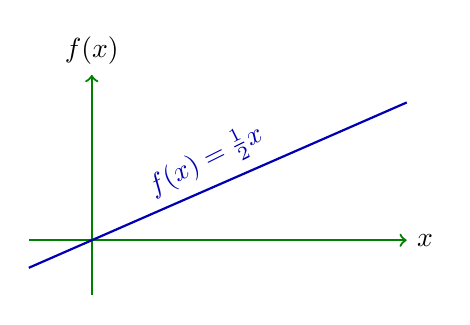
\begin{tikzpicture}
[
	xscale	= 0.8,	% to scale horizontally everything but the text
	yscale	= 0.7,	% to scale vertically everything but the text
]


\draw [->, color=black!50!green, thick] (-1,0) -- (5,0) node [right, color=black] {$x$};
\draw [->, color=black!50!green, thick] (0,-1) -- (0,3) node [above, color=black] {$f(x)$};
\draw [-, color=blue!70!black, thick] (-1,-0.5) -- (5,2.5) node [midway, above, sloped] {$f(x) = \frac{1}{2} x$};


\end{tikzpicture}
\end{center}
\end{figure}
 

	%
\end{frame}






\begin{frame}
	%
	\frametitle{Paths: how to set their terminations}
	%
	(example file: \url{./Sources/paths__caps_usage.tex} - requires \texttt{arrows} library)
	%
	

\begin{figure}[!htb]
\begin{center}
\begin{tikzpicture}
[
	xscale	= 1,	% to scale horizontally everything but the text
	yscale	= 1,	% to scale vertically everything but the text
]


\uncover<1->
{
	% not requiring ``arrows'' library
	\draw [ultra thick, ->]		(0,0) -- (1,2);
	\draw [ultra thick, >->>]	(1,0) -- (2,2);
	\draw [ultra thick, |<->|]	(2,0) -- (3,2);
}





\uncover<2->
{
	% requiring ``arrows'' library
	\draw [ultra thick, [-triangle 90]		(4,0) -- (5,2);
	\draw [ultra thick, hooks-open diamond]	(5,0) -- (6,2);
	\draw [ultra thick, left hook reversed-square]	(6,0) -- (7,2);
}


\end{tikzpicture}
\end{center}
\end{figure}




	%
\end{frame}






\begin{frame}
	%
	\frametitle{How to position text along a path}
	%
	(example file: \url{./Sources/paths__text_positioning.tex})
	%
	\begin{figure}[!htb]
\begin{center}
\begin{tikzpicture}
[
	xscale	= 0.8,	% to scale horizontally everything but the text
	yscale	= 0.9,	% to scale vertically everything but the text
]





\uncover<1->
{
	% intuitive positioning
	\draw
	[
		color	= blue!40,
		thick,
		-open triangle 45
	]
	(0,0) -- (2,5)
	node[black, at end]				{this is at the end}
	node[black, near end]			{this is at the near end}
	node[black, midway]				{this is at the midway}
	node[black, very near start]	{this is at the very near start};
}







\uncover<2->
{
	% numerical positioning
	\draw
	[
		color	= red!50,
		ultra thick,
		dotted,
		-open triangle 45
	]
	(5,0) -- (7,5)
	node[black, pos=0.0]			{this is at position 0.0}
	node[black, pos=0.3]			{this is at position 0.3}
	node[black, pos=0.5]			{this is at position 0.5}
	node[black, pos=1.1]			{this is at position 1.1};
}






\uncover<3->
{
	% sloping
	\draw
	[
		color	= black!30!orange,
		thick,
		-open triangle 45
	]
	(-2,2) -- (-5.0,6.5)
	node
	[				% here we define some properties of the node!
		midway,
		sloped,
		above,
		color = black!30!orange
	]
	{sloped text};
}




\end{tikzpicture}
\end{center}
\end{figure}

	%
\end{frame}

 



\begin{frame}
	%
	\frametitle{How to decorate paths}
	%
	(example file: \url{./Sources/paths__decorations.tex})
	%
	\begin{figure}[!htb]
\begin{center}
\begin{tikzpicture}
[
	xscale	= 1,	% to scale horizontally everything but the text
	yscale	= 1,	% to scale vertically everything but the text
]



\uncover<1->
{
	% text along a path
	\draw
	[
		decorate,
		decoration =
		{
			text along path,
			text color	= blue,
			text		= This is a text along a path. Note how some portion of the path is lost.
		}
	]
	(0,0) .. controls (3,3) and (9,3) .. (9,0);
}


\uncover<2-2>
{
	\node [circle, fill = gray, minimum size = 3mm] at (0,0) {};
	\node [circle, fill = gray, minimum size = 3mm] at (3,3) {};
	\node [circle, fill = gray, minimum size = 3mm] at (9,3) {};
	\node [circle, fill = gray, minimum size = 3mm] at (9,0) {};
	\draw
	[
		line width	= 0.1cm,
		color		= red,
	]
	(0,0) .. controls (3,3) and (9,3) .. (9,0);
}



\uncover<4->
{
	\node
	[
		draw,
		thick,
		minimum height	= 2cm,
		minimum width	= 3.5cm,
		fill			= yellow!50,
		inner xsep		= 0.3cm,
		inner ysep		= 0.3cm,
		decorate,
		decoration =
		{
			random steps,
			segment length	= 0.1cm,
			amplitude		= 0.09cm
		}
	]
	at (4.5,-1)
	{Saved from trash};
}



\end{tikzpicture}
\end{center}
\end{figure}


	%
\end{frame}


 
 
 
